\documentclass{article}

\usepackage[UTF8]{ctex}
\usepackage{amsmath,amssymb}
\usepackage{geometry}
\usepackage{graphicx}

\geometry{a4paper, margin=2.5cm}

\begin{document}

% ============================================================
\section*{n 步回报}

\subsection*{先讲一个故事}

你已经知道了 DQN 和 A2C/PPO。回头看它们的更新目标：

\[
\underbrace{r_{t+1} + \gamma \max_{a'} Q(s_{t+1}, a')}_{\text{DQN 的目标（1步 bootstrap）}}
\qquad\qquad
\underbrace{\sum_{k=0}^{T-t-1} \gamma^k r_{t+k+1}}_{\text{REINFORCE 的目标（完整 MC 回报）}}
\]

两个极端。A2C 引入 GAE，PPO 默认 $\lambda=0.95$——它们都在做同一件事：在「只看一步」和「看完整条轨迹」之间找一个折中点。

\textbf{这个折中点的名字，就是 n 步回报。}

它是 DQN、A2C、PPO 共同的地基，在我们写出那些算法之前就应该先讲清楚的东西。今天倒回来把这块砖补上。

\subsection*{数学形式化}

从状态 $s_t$ 出发，沿真实轨迹走 $n$ 步，再用价值函数对 $s_{t+n}$ 做 bootstrap：

\[
\boxed{G_t^{(n)} = \sum_{k=0}^{n-1} \gamma^k r_{t+k+1} \;+\; \gamma^n\, V(s_{t+n})}
\]

\begin{itemize}
  \item 前半段 $\sum \gamma^k r_{t+k+1}$：$n$ 步真实奖励，无偏但带随机性；
  \item 后半段 $\gamma^n V(s_{t+n})$：从第 $n$ 步起的估计价值，快速但依赖网络精度；
  \item $n=1$ 退化为 TD(0)（DQN 的目标）；$n \to \infty$ 退化为 MC 回报（REINFORCE 的目标）。
\end{itemize}

% ============================================================
\section*{偏差与方差：两步之间的取舍}

\subsection*{bootstrap 带来的偏差}

$G_t^{(1)}$ 把未来的所有不确定性「外包」给了 $V(s_{t+1})$：

\[
G_t^{(1)} = r_{t+1} + \gamma \cdot \underbrace{V(s_{t+1})}_{\text{训练初期精度有限}}
\]

如果 $V$ 尚未收敛，bootstrap 值会把网络当前的估计误差直接拉进训练目标。$n=1$ 对 $V$ 的精度最敏感——它把所有未来折扣奖励全部交给 $V$ 来代理。

多走 $n$ 步之后，bootstrap 的影响被 $\gamma^n$ 压缩：

\[
\text{偏差} \;\propto\; \gamma^n \cdot \bigl\|V_\theta(s_{t+n}) - V^*(s_{t+n})\bigr\|
\;\xrightarrow[]{n \uparrow}\; 0
\]

$\gamma=0.99$，$n=16$：$\gamma^{16} \approx 0.85$，bootstrap 的影响已缩减近 $15\%$。如果实验中 episode 较短，甚至不需要考虑bootstrap的缩减影响，$n=16$ 往往直接退化为 MC 而无需 bootstrap。

\textbf{注意}：这并不意味着 $n=1$ 不能收敛。DQN 正是用 $n=1$ 的 TD(0) 目标，配合高频 target 网络同步（每 $100$ 步一次）和大容量 replay buffer，将 bootstrap 偏差控制在可接受范围内——工程设施弥补了理论上的敏感性。

\subsection*{Monte Carlo 带来的方差}

$G_t^{(\infty)}$ 完全依赖真实奖励，bootstrap 权重为零，偏差为零。但 $T-t$ 个随机变量叠加：

\[
\mathrm{Var}\!\left[G_t^{(\infty)}\right] = \sum_{k=0}^{T-t-1} \gamma^{2k} \cdot \mathrm{Var}[r_{t+k+1}]
\]

轨迹越长，方差越大，梯度信号越嘈杂。

\subsection*{实验验证：从同一起点出发的 400 条轨迹}

\begin{figure}[htbp]
  \centering
  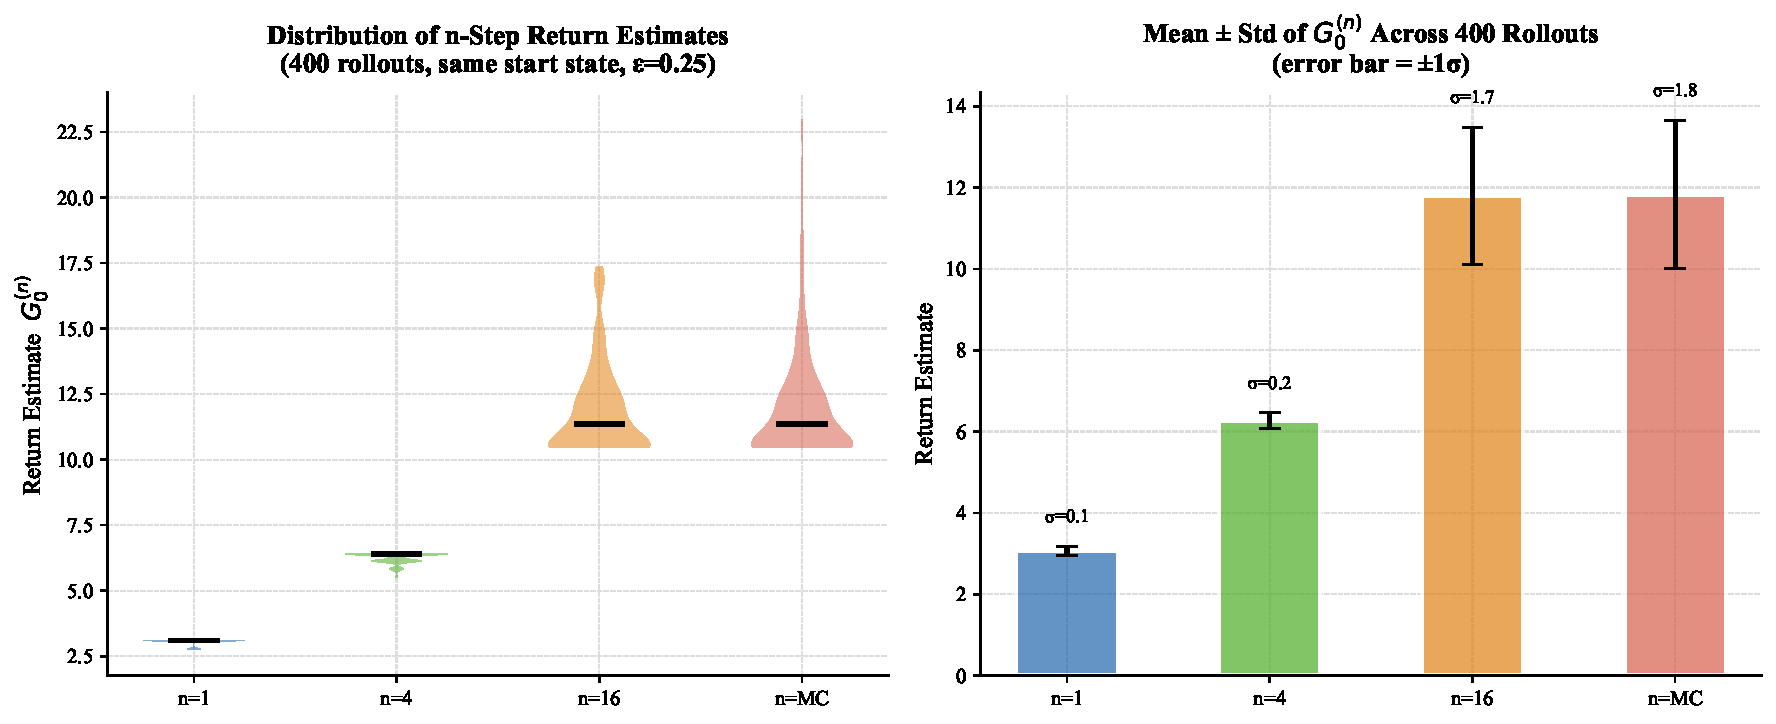
\includegraphics[width=\textwidth]{fig2_variance_bias.pdf}
  \caption{从固定初始状态出发，$\varepsilon$-greedy（$\varepsilon=0.25$）采集 400 条轨迹，
           计算各 $n$ 步回报估计 $G_0^{(n)}$ 的分布。
           Bootstrap 使用仅训练 100 episode 的参考网络（体现早期偏差）。
           \textbf{左}：分布形态，方差随 $n$ 递增清晰可见；
           \textbf{右}：均值 $\pm 1\sigma$，n=1 均值（3.06）远低于 MC（11.83），偏差显著。}
\end{figure}

\[
\begin{array}{c|c|c|l}
n & \text{均值} & \text{标准差（$\sigma$）} & \text{解读} \\
\hline
1    & 3.06  & 0.10 & \text{强偏向网络估计，极低方差，高偏差} \\
4    & 6.26  & 0.19 & \text{偏差减半，方差仍低} \\
16   & 11.80 & 1.69 & \text{接近真实价值，方差升高} \\
\text{MC} & 11.83 & 1.83 & \text{无偏，但方差最大} \\
\end{array}
\]

n=1 的均值（3.06）远低于 MC（11.83），正是因为参考网络在早期把价值严重低估，bootstrap 把这个错误拉进了估计里。n=16 和 MC 均值几乎一致，说明偏差已经消除。

% ============================================================
\section*{n 步回报对训练动态的影响}

\subsection*{学习曲线：n=1 卡死，n=16 收敛}

\begin{figure}[htbp]
  \centering
  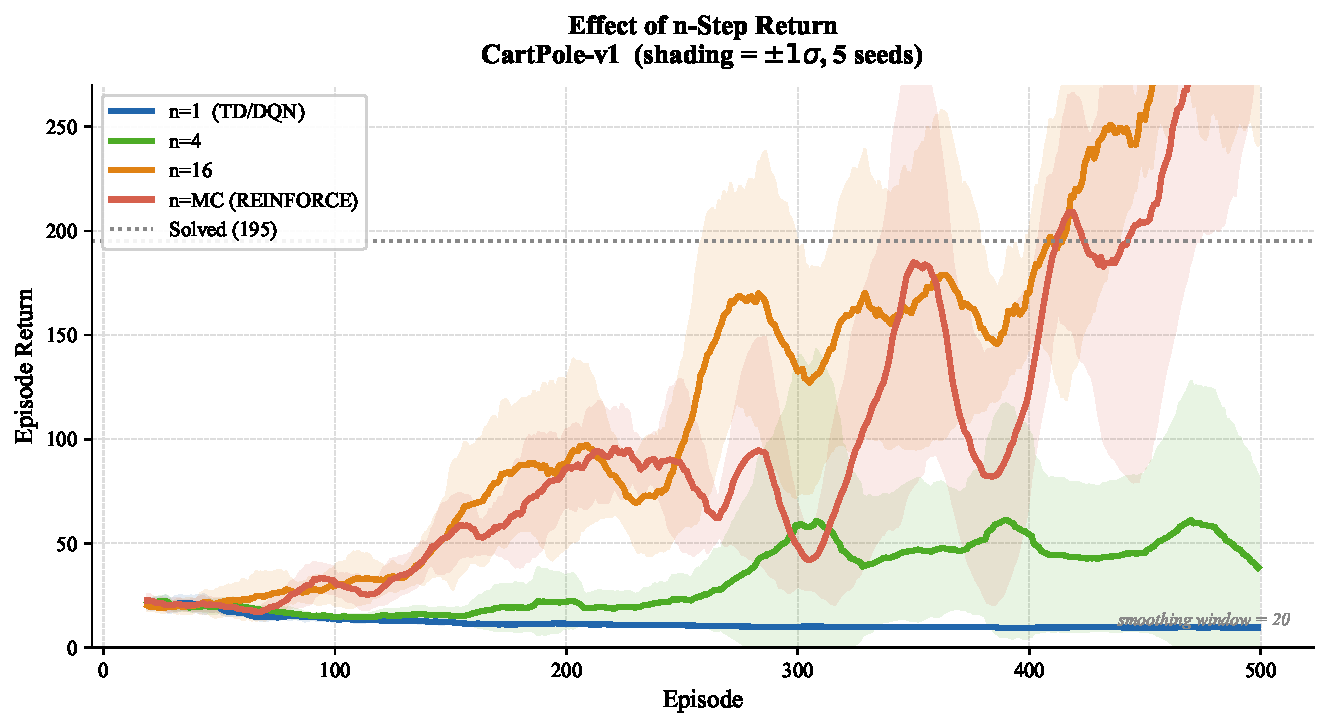
\includegraphics[width=\textwidth]{fig1_nstep_curves.pdf}
  \caption{CartPole-v1，各 $n$ 步 Q-learning 学习曲线（5 个随机种子，$\pm 1\sigma$ 阴影，平滑窗口=20）。
           n=1 全部种子卡死在 $\approx 9.9$（随机水平）；n=4 部分种子学习；n=16 和 MC 均收敛至 200 以上。}
\end{figure}

n=1 在本实验中卡死的机制：

\begin{enumerate}
  \item 实验中 target 网络每 $20$ 个 episode 才同步一次（而非 DQN 的每 100 步），
        早期 $G_t^{(1)} = r + \gamma V_\theta(s')$ 长期使用不准确的 bootstrap；
  \item 这些偏差目标积压在 replay buffer，混入后续所有 mini-batch；
  \item $Q$ 网络被拉向错误方向，target 网络同步后继承偏差，循环难以自我纠正。
\end{enumerate}

这是实验设定放大了 n=1 的敏感性，而非 n=1 本身不可行。DQN 用更密集的 target 同步策略解决了同一问题。

n=16 在本实验中幸免于难：早期 episode 平均只有约 9 步，$n=16 > T$，实际退化为完整 MC 回报，无需 bootstrap，因此对 target 网络精度完全免疫。

\textbf{翻译成人话}：靠自己多走几步，就不那么需要依赖一个还没学好的老师给的答案。

\subsection*{CartPole 之外：更长 episode 里的甜点}

CartPole 的 episode 很短（约 9 步），任意 $n \ge 9$ 都退化为 MC，因此 Fig 1 只能看出「n=1 vs 其余」的二分。在 episode 长达数千步的环境里（可以去看一看 Rainbow 那篇论文），偏差-方差的折中才真正显现：$n=3$ 时 bootstrap 权重 $\gamma^3 \approx 0.97$，bootstrap 依赖已有所压缩，而方差远小于完整 MC 回报——这是在更长 episode 任务上实践验证的折中点。

% ============================================================
\section*{TD($\lambda$)：把 $n$ 软化成连续参数}

\subsection*{前向视角：对所有 $n$ 步回报做加权平均}

不固定单一的 $n$，而是用 $\lambda \in [0,1]$ 对所有 $n$ 步回报做指数加权平均：

\[
\boxed{G_t^\lambda = (1-\lambda) \sum_{n=1}^{\infty} \lambda^{n-1}\, G_t^{(n)}}
\]

权重 $(1-\lambda)\lambda^{n-1}$ 以 $\lambda$ 为公比递减，短步权重高。$(1-\lambda) \sum_{n=1}^\infty \lambda^{n-1} = 1$，权重归一。

\subsection*{后向递推：代码里真正用的形式}

前向视角需要知道整条未来轨迹，无法在线高效计算。等价的后向递推从轨迹末尾反向扫描一遍即可：

\[
\boxed{G_t^\lambda = r_{t+1} + \gamma\bigl[(1-\lambda)\,V(s_{t+1}) \;+\; \lambda\, G_{t+1}^\lambda\bigr]}
\]

边界条件：$G_T^\lambda = r_T$（终止状态无后继，无需 bootstrap）。

\textbf{验证两极端}：
\begin{itemize}
  \item $\lambda=0$：$G_t^0 = r_{t+1} + \gamma V(s_{t+1})$，纯 TD(0) 目标 \checkmark
  \item $\lambda=1$：$G_t^1 = r_{t+1} + \gamma G_{t+1}^1$，标准 MC 回报递推 \checkmark
\end{itemize}

\subsection*{TD($\lambda$) 实验结果}

\begin{figure}[htbp]
  \centering
  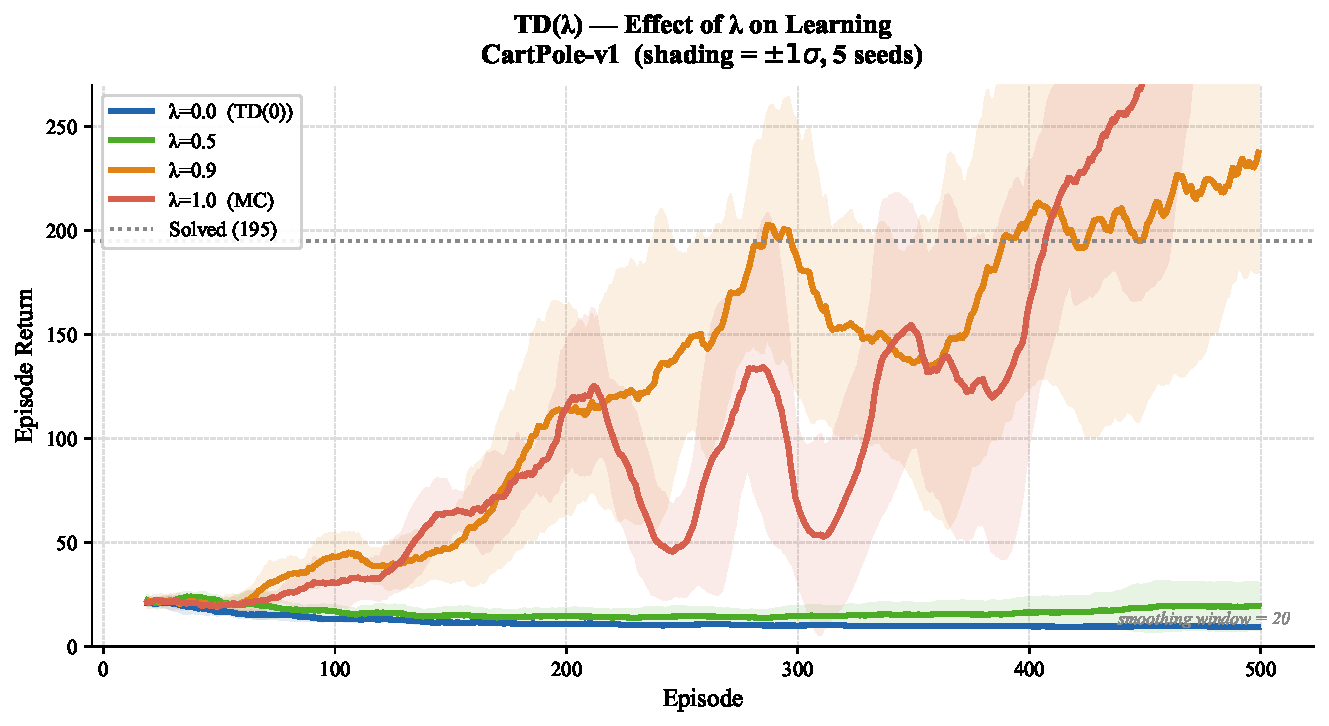
\includegraphics[width=\textwidth]{fig3_lambda_return.pdf}
  \caption{CartPole-v1，四种 $\lambda$ 值的 TD($\lambda$) Q-learning（5 个种子，$\pm 1\sigma$，平滑窗口=20）。
           $\lambda=0$ 与 n=1 行为完全一致，全部卡死；$\lambda=1.0$ 即 MC 表现最优。}
\end{figure}

\[
\begin{array}{c|l|c}
\lambda & \text{含义} & \text{last-50 平均回报} \\
\hline
0.0 & \text{纯 TD(0)，完全依赖 bootstrap} & \approx 9.6 \text{（卡死）} \\
0.5 & \text{中等权重，仍高度依赖 bootstrap} & 11 \sim 41 \text{（不稳定）} \\
0.9 & \text{偏重长步，bootstrap 依赖少} & 158 \sim 324 \text{（收敛）} \\
1.0 & \text{纯 MC，完全不用 bootstrap} & 298 \sim 415 \text{（最优）} \\
\end{array}
\]

结论与 Fig 1 一致：$\lambda$ 越高，对 bootstrap 依赖越少，早期训练越稳定。

% ============================================================
\section*{与 GAE 的关系}

A2C 和 PPO 里的 \textbf{GAE（广义优势估计）} 是 TD($\lambda$) 在优势函数上的直接应用。

定义 TD 误差 $\delta_t = r_{t+1} + \gamma V(s_{t+1}) - V(s_t)$，则：

\[
\boxed{A_t^{\mathrm{GAE}(\lambda)} = \sum_{l=0}^{T-t-1} (\gamma\lambda)^l\, \delta_{t+l}}
\]

\textbf{翻译成人话}：GAE 把一串 TD 误差用 $\gamma\lambda$ 指数衰减地加起来。$\lambda=1$ 把所有步全加完（$\approx$ MC 优势）；$\lambda=0$ 只用当步误差（$= $ 1步 TD 优势）。

PPO 默认 $\lambda=0.95$ 的含义：网络已具备一定精度，此时适度降低 MC 依赖（略小于 1）可以压缩方差，加速后期收敛。

% ============================================================
\section*{四种估计方式的横向对比}

\[
\begin{array}{c|c|c|c|c}
\text{方法} & \text{公式} & \text{偏差} & \text{方差} & \text{典型应用} \\
\hline
\text{TD(0)}    & r+\gamma V(s')                       & \text{高（依赖 }V\text{）} & \text{低}  & \text{DQN } (n{=}1) \\
n\text{-step}   & \sum_{k<n}\gamma^k r_{k+1}+\gamma^n V & \text{中}                  & \text{中}  & \text{实践中常用 } n{=}3{\sim}10 \\
\text{MC}       & \sum_k \gamma^k r_{k+1}              & \text{零}                  & \text{高}  & \text{REINFORCE} \\
\text{TD}(\lambda) & (1-\lambda)\sum_n \lambda^{n-1} G^{(n)} & \text{可调}           & \text{可调} & \text{GAE in PPO ($\lambda{=}0.95$)} \\
\end{array}
\]

\subsection*{为什么实践中偏向大 $n$ 或大 $\lambda$？}

\begin{enumerate}
  \item \textbf{早期训练}：$V$ 还不准，bootstrap 危险。大 $n$ / 大 $\lambda$ 减少对 $V$ 的依赖，学习更稳定——这是本章实验的核心发现。
  \item \textbf{后期训练}：$V$ 已经较准，MC 的高方差反而拖慢收敛。适度减小 $n$ 或 $\lambda$ 降低方差——PPO 用 $\lambda=0.95$ 而非 1.0，即出于此考量。
  \item \textbf{折中的本质}：并无理论最优，中等 $n$ 和 $\lambda=0.95$ 均为实践中多任务验证的稳健值。
\end{enumerate}

% ============================================================
\section*{本章在 RL 体系中的位置}

n 步回报是一块被后来算法反复引用、却没有被单独讲清楚的地基：

\begin{enumerate}
  \item \textbf{TD 路线} $\to$ TD(0) $\to$ $n$\text{-step TD} $\to$ DQN（$n=1$）：
        这条线一路都是 bootstrap，区别在于用多少步真实奖励来稀释 bootstrap 的影响，
        以及用什么工程手段（target 网络、replay buffer）控制偏差。
  \item \textbf{MC 路线} $\to$ REINFORCE $\to$ Actor-Critic：
        MC 回报（$n=\infty$）是 REINFORCE 的基础，消除方差是从 MC 到 AC 的核心动机。
  \item \textbf{$\lambda$ 路线} $\to$ TD($\lambda$) $\to$ GAE $\to$ PPO/A2C：
        $\lambda$ 把离散的 $n$ 连续化，GAE 把它用在优势函数上，PPO/A2C 默认 $\lambda=0.95$。
\end{enumerate}

\underline{一个值得思考的问题}：DQN 选了 $n=1$，而非 MC——为什么在 episode 足够长的环境里，MC 回报反而不是更好的选择？

\subsection*{参考资料}

\begin{enumerate}
  \item Sutton \& Barto (2018). \textit{Reinforcement Learning: An Introduction} (2nd ed.). Chapter 7: $n$-step Bootstrapping.
  \item Mnih et al.\ (2015). Human-level control through deep reinforcement learning. \textit{Nature}. （DQN 原论文，$n=1$）
  \item Schulman et al.\ (2016). High-dimensional continuous control using generalized advantage estimation. \textit{ICLR}. （GAE 原论文，TD($\lambda$) 的优势函数版本）
  \item Mnih et al.\ (2016). Asynchronous methods for deep reinforcement learning. \textit{ICML}. （A3C，$n$-step target 的实践应用）
\end{enumerate}

\end{document}
